\section{Normality Test}

In our analysis part, we use linear model to fit real data. There are several
assumptions on linear modeling, one of which is normality assumption on error 
term. Normality of the errors can be checked by checking normality of the 
residuals. The usual way is to draw a Q-Q plot and check whether it forms a 
straight line. However in this paper, since there are around 200,000 voxels,
it would be hard to plot all of them and check for normality. Thus we use 
Shapiro-Wilk test in the paper to test for normality. \par

In Shapiro-Wilk test, a small p-value indicates non-linearity. We write a
function to compute p-value of each voxel and plot those p-values in three
brain perspectives. There are three linear models used in the paper. The 6 
plots below are p-value plots: the three plots to the left are p-values for three 
different linear models using raw data. The other three plots are p-values for 
three different linear models using smoothed data. \par

\begin{figure}[ht]
\begin{subfigure}{.52\textwidth}
  \centering
  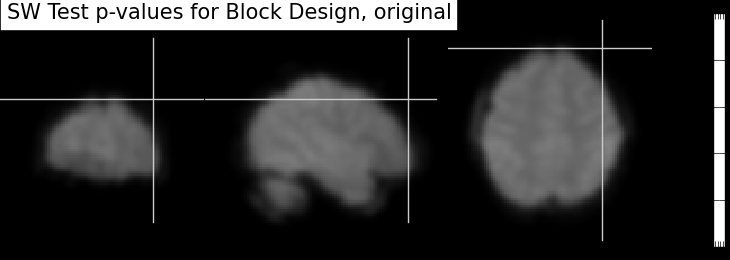
\includegraphics[scale=0.42]{block_normality_test}
\end{subfigure}%
\begin{subfigure}{.4\textwidth}
  \centering
  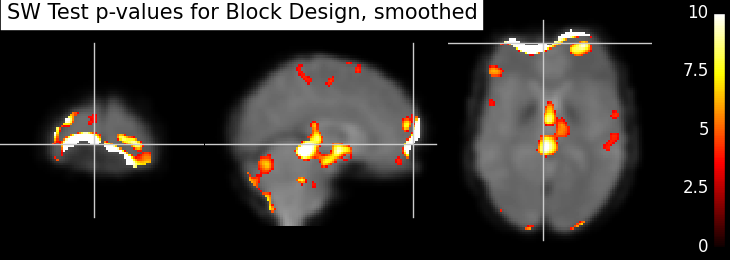
\includegraphics[scale=0.42]{smoothed_block_normality_test}
\end{subfigure}
\begin{subfigure}{.52\textwidth}
  \centering
  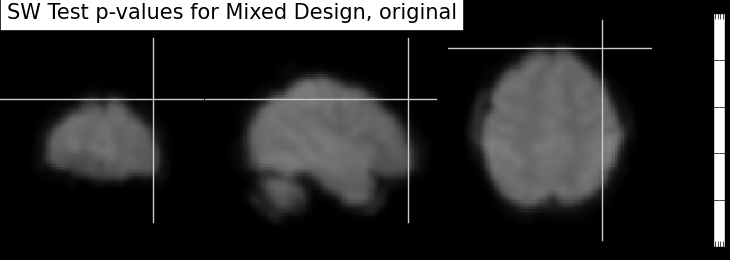
\includegraphics[scale=0.42]{mixed_normality_test}
\end{subfigure}%
\begin{subfigure}{.4\textwidth}
  \centering
  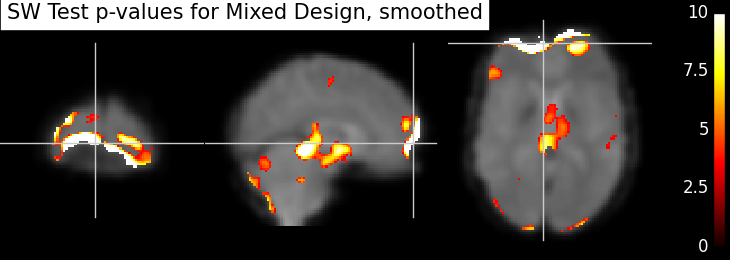
\includegraphics[scale=0.42]{smoothed_mixed_normality_test}
\end{subfigure}
\begin{subfigure}{.52\textwidth}
  \centering
  
\includegraphics[scale=0.42]{mixed_dct_normality_test}
\end{subfigure}%
\begin{subfigure}{.4\textwidth}
  \centering
  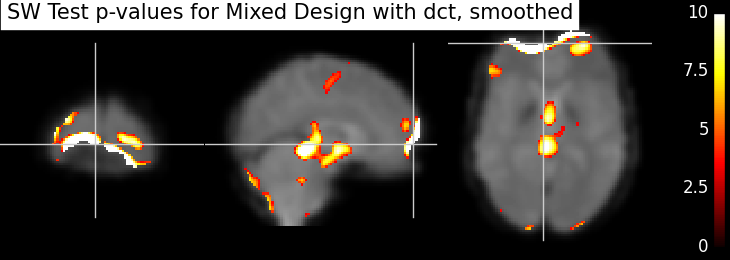
\includegraphics[scale=0.42]{smoothed_mixed_dct_normality_test}
\end{subfigure}
\caption{SW Test for Three Linear Models\label{fig:swtest}}
\end{figure}

The bright areas in the above plots means errors in that area don't follow
normal distribution. We can see that data before smoothed seems to follow
normal distribution well, while data after smoothing show some non-normality.
This makes sense because there should be significant points for anatomy.





